\documentclass[a4paper,english]{report}
\usepackage[utf8]{inputenc}
\usepackage{babel,duomasterforside}
\usepackage{color}   %May be necessary if you want to color links
\usepackage{hyperref}
\usepackage{svg}
\usepackage{graphicx,wrapfig,lipsum}
\hypersetup{
	colorlinks=true, %set true if you want colored links
	linktocpage=true,     %set to all if you want both sections and subsections linked
	linkcolor=blue,  %choose some color if you want links to stand out
}

\title{Performance tuning Apache Drill on Hadoop Clusters with Genetic Algorithms}
\subtitle{Improving industry standards for advanced analytics and business intelligence}
\author{Roger Bløtekjær}

\begin{document}
	\duoforside[dept={Institutt for informatikk},
	program={Informatikk: språkteknologi},
	short]
	\section{Abstract}
		\subsection{Research question}
		How can we make a self optimizing distributed Apache Drill cluster, for high performance data readings across several file formats and database architectures?
		\subsection{Overview}
		Apache has introduced a new building block that's best suited on top of the Hadoop Stack called Apache Drill. Drill enables the user to perform schema-free querying of distributed data, and ANSI SQL programming on top of NoSQL datatypes like JSON or XML. As it is with the core Hadoop stack, Drill is also highly customizable, with plenty of performance tuning parameters to ensure optimal efficiency. Tweaking these parameters however, requires deep domain knowledge and technical insight, and even then the optimal configuration may not be evident. Businesses will want to use Apache Drill in a Hadoop cluster, without the hassle of configuring it, for the most cost-effective implementation. This can be done by solving the following problems:
		\begin{itemize}
			\item How to apply genetic algorithms in the most cost-effective way to automatically tune a distributed Apache Drill configuration, regardless of cluster environment.
			\item How do we benchmark the cluster against default Drill settings, as well as known SQL performance tests, to ensure that the algorithm is adding value to the cluster performance, measured as execution time.
		\end{itemize}
		\subsection{Details}
			\subsubsection{Self optimizing}
			The goal here is that no human intervention is needed to fine tune the Drill configuration. Once the framework / algorithm is executed on the Drill environment, it should only end execution when performance is proven to be optimized.
			\subsubsection{Genetic Algorithms}
			The methodology for self optimization in this thesis is genetic algorithms. A branch of evolutionary algorithms that rely on randomly distributed properties given to a population of candidates. The properties are hereditary and define the next generation of candidates, eventually resulting in a "proven optimal candidate", to solve a given problem.
			\subsubsection{Distributed file systems / cluster environments}
			Apache Drill can easily be run on any file system, as they are mounted when needed. As such a single node environment is entirely possible to set up, with the local file system mounted as a "Drill Bit". However this thesis focuses on current and future industry standards, and how to optimize Drill in a relevant a big data environment. This is more representative of its intended use, and gives the thesis more value as a research field advancement.
			\subsubsection{ANSI SQL}
			There are similar platforms to Apache Drill, like the popular Apache Spark. Spark also provides SQL querying on data, however this is only a subset of SQL. Only Drill has the full suit of SQL programming capabilities as defines by ANSI (American National Standards Institute), which gives more in depth querying.
			\subsubsection{NoSQL}
			Previously NoSQL databases where known as "Non-SQL" databases, but this has now changed to be "Not Only SQL" databases as they have begun supporting SQL-like querying. The main point about them is that they are non-relational, distributed, open-source and horizontally scalable\cite{no_sql}.
	
	\pagebreak
	\section{Foreword}
	Can be omitted if I want, keeping it for now.
	
	\tableofcontents
	
	\chapter{Preface}
	\section{List of figures}
	\section{List of tables}
	\section{Abbreviations}
	\label{word_list}
	\begin{table}[h]
		\centering
		\begin{tabular}{ll}
			TTE	& Time to execute \\
			OOP	& Object Oriented Programming \\
			HDFS & Hadoop Distributed File System \\
			PBIL & Population Based Incremental Learning \\
			GA & Genetic Algorithms \\
			ER & Entity Relation \\
			SMB & Small / Medium Business \\
			SQL EE & Structured Query Language Execution Engine \\
			MPP & Massively Parallel Processing \\
			RPC & Remote Procedure Call \\
			DSN & Data Source Name \\
		\end{tabular}
	\end{table}

	
	\chapter{Introduction}
		
		\section{Target group}
		This thesis covers the deep technical aspects of big data analysis and genetic algorithms - However, all techniques used will be explained in detail. Computer science students looking into infrastructure will probably feel the most at home, in terms of discussed concepts and technical terms. For the layman, there is also a \hyperref[word_list]{word list} supplied with brief explanations for technical terms used in this thesis.
		
		\section{Area of research}
		Hadoop and MapReduce are already well established technologies employed in countless applications around the world, Apache Drill however is a fairly new concept with little to no research from the community. We propose a new method of implementing Hadoop clusters with Apache Drill, automatically optimizing the performance tuning in a lightweight and low effort way. As such this is a technical thesis regarding performance tuning, and the implementation aspects of an Apache Drill cluster.
		
		\section{Research question - in full}
		\subsection{Goal, justification and challenges}
		The goal for this thesis is to optimize a SQL Engine that sits on top of a distributed storage, for more cost-effective big data handling, business intelligence and advanced analytics. Businesses that handle big data will most likely perform plenty of queries every day, or even every hour. If we were to add up the amount of time spent waiting for a query to complete, for a year, and converted the hours into money - we would find it costs a lot of money to convert raw data into information. That's why saving even 10\% in execution time can mean a big difference when it comes to overhead costs. So naturally there is a massive amount of research for improving execution time and other metrics, even more so when it comes to shared computing like cloud services where you pay by the minute. The SQL Engine chosen here is Apache Drill, a fairly new framework inspired by Google Dremel, and currently the only schema-free engine to run on top of HDFS, allowing users to drill into complex data like JSON. Looking to for example Yelp, we can see that their entire database is available as JSON\cite{yelp}, allowing for far more complex  and flexible handling of metrics than conventional ER databases. As with the other data handling engines on distributed storage platforms, there are many parameters to consider if one wants to increase performance - in fact so many that it is considered infeasible without in depth expertise of domain and engine. Considerations are:
		\begin{itemize}
			\item Type of storage (distributed or single node)
			\item Amount of computing nodes (cluster or not)
			\item Size of nodes (memory and CPU)
			\item Type of data (complex or not)
			\item Size of data (few large files or plenty small ones)
			\item Distribution of data (heavy skew or uniform distribution)
			\item Execution engine specific parameters (for which there are many)
		\end{itemize}
		All of these parameters work in tandem to produce a measurable performance. That's why genetic algorithms was chosen as a tool for self optimization, to take all of these parameters into consideration automatically - and simply test solutions until converging into a good one (considered optimal). Some of the parameters are statically set in this thesis, such as cluster size, to simulate a SMB environment, and to have some testing grounds. There would be no alterations needed to apply the methods presented in this thesis in either an enterprise with 1000 clustered nodes, or a single laptop, but for the sake of argument we mimic a real world use case.
		\subsection{Resarch question}
		How can we make a self optimizing distributed Apache Drill cluster, for high performance data readings across several file formats and database architectures?
		
		\section{Personal motivation}
			\subsubsection{Subject}
			The subject for this master thesis is a natural continuation of our previous work \emph{Hadoop MapReduce Scheduling Paradigms}, published in 2017, in the 2nd IEEE International Conference on Cloud Computing and Big Data Analysis (ISSSBDA 2017). Back then the topic was haphazardly picked from a list of eligible ones, but the more we read into it - the more we understood the incredible use cases for Hadoop within the massive industries that are driving forces for our technological advancements. As is common in IT, levels of abstraction get added on top of proven technologies both to make implementation better, and often to increase performance. Since then Apache Drill has seen plenty of stable builds and proven itself to be potentially industry-changing in the way we handle our data - entering a schema-on-the-fly paradigm.
			\subsubsection{Apache Drill as a platform}
			As mentioned previously there is little to no research done on Apache Drill as a platform. Some of the reasoning might be the that some still considers it to be in the early development phase, but as of this writing there has already been one major release, \textbf{1.0} in 2015, and 12 subsequent minor releases up till \textbf{1.12}\cite{drill_releases}. So we would argue the project is past the early development phase, and moving into the early adopter phase. But why choose to use this platform over more established ones, and what other options are there? This is discussed further in a following section: \hyperref[sec:why_drill]{Why is this worthwhile?}
		
		\section{Research method in brief}
		Throughout this thesis we will develop an entire suite of tools centered around a genetic algorithm for automatically optimizing Apache Drill on top of a Hadoop cluster, tested on big and diverse sample sets. As the framework is expected to change, all of the parameters tweaked will be in relation to the current version being used, \textbf{1.12}. The main goal is to achieve a performance increase, measured as TTE (Time to Execute) for single and/or concurrent queries. Examining previous studies on SQL performance will provide a good basis for best practices within SQL query execution optimization, and how to measure it.
		
		\section{Most relevant previous findings}
		There is little to no research done on the impact of tuning Apache Drill. However, tuning of parameterized frameworks have been done a lot in the past on industry standards like SQL, MySQL, traditional Hadoop clusters (mapreduce scheduling algorithms), and Web applications. Since Apache Drill has its own SQL execution engine,  the tuning of SQL systems in previous works has value for how we will benchmark our Drill perfomance.
			\subsection{Starfish}
			Herodotos et al made on of the most cited papers in the Hadoop research field, when they proposed Starfish \cite{starfish}. Starfish is a self-tuning system for Hadoop clusters, citing the lackluster performance of default cluster parameters to be the motivation. They designed a modular system where the main parts include:
			\begin{itemize}
				\item A profiler that analyzes jobs and determines cost estimation and the data flow.
				\item A novel approach to predictive tuning they named the "what-if-engine". It's job is to predict how different parameter configuration tweaks will change the performance of the system.
				\item A cost-based optimizer, that performs the pure tuning aspects, based on estimations from the what-if-engine.
			\end{itemize}
			Our project has very similar goals and motivations compared to this project, except on a framework on top of Hadoop, instead of directly on it.
		
		\section{Why is this worthwhile, why Drill?}
		\label{sec:why_drill}
			\subsection{Ease of use}It is safe to say that information technology as a subject is only getting more popular by demand. According to projections made by renown recruitment company Modis, tech employment will see a 12\% growth by 2024, vs 6,5\% in all other industries\cite{modis}. This means that a lot of new engineers will enter the workforce, and start building and maintaining enterprise applications. Apache Drill serves a very low barrier of entry for newcomers with its' SQL ANSI queries when handling big amounts of data, as opposed to i.e the popular Java Enterprise framework Persistence. Using Apache Drill will therefore require less training, thus increasing productivity and agility in young teams.
			\subsection{Increasing relevance of Big Data infrastructures}
			\label{big_data}
			\textit{"From 2005 to 2020, the digital universe is expected to grow dramatically by a factor of 300, from 130 exabytes to 40 trillion gigabytes, i.e more than 5,200 gigabytes per person in 2020. Moreover, the digital universe is expected to double every two years"}\cite{bigdata}.
				\subsubsection{Real time data usage}
				Successful digitalization of businesses often require applications to utilize data in real time, serving customers relevant data instantaneously. \textit{"Now, most applications are generating real-time data, so superfast data capturing and analysis within a fraction of a second are mandatory"}\cite{management_analytics}.
				\\
				An interesting example of this is chat applications (instant messaging). Users of messaging apps today expect it to store data indefinitely, and deliver instant communication between users, creating an absolutely enormous global data flow. Bettercloud.com performed a study and found that\cite{bettercloud}:
				\begin{itemize}
					\item The majority of organizations (57\%) use two or more real-time messaging applications.
					\item 80\% of Skype for Business users, 84\% of Google Hangouts users, and 95\% of Slack users say communication has improved because of real-time messaging.
					\item 56\% of respondents believe that real-time messaging will displace email as their organization’s primary workplace communication and collaboration tool.
				\end{itemize}
				From these results we see that adoption of applications using real time data is only increasing. This will provide a future need for fast and scalable infrastructure to cope with it. 
				\subsubsection{Combining real-time and stored data}
				In reality a lot of current applications that create value combine the usage of analytics on stored data and real-time sensor data. Predictive maintenance is an example of a discipline where you analyze historical data, finding thresholds and patterns for when components in a system break down, and then combining this knowledge with real time sensors to service the components before they fail. This saves money on planned maintenance where healthy parts get serviced, and downtime on systems where they have to be set aside for the service. In a Harvard Business Review on a company called \textbf{Servicemax} that has specialized in services like this they wrote that:
				\textit{"(...) customers, on average, increase productivity by 31\%, service revenue by 14\% and customer satisfaction by 16\%"}\cite{servicemax}. All of this is empowered by big data, and the utilization of information.
			
			\subsection{Application needs}
			\begin{figure}[h]
					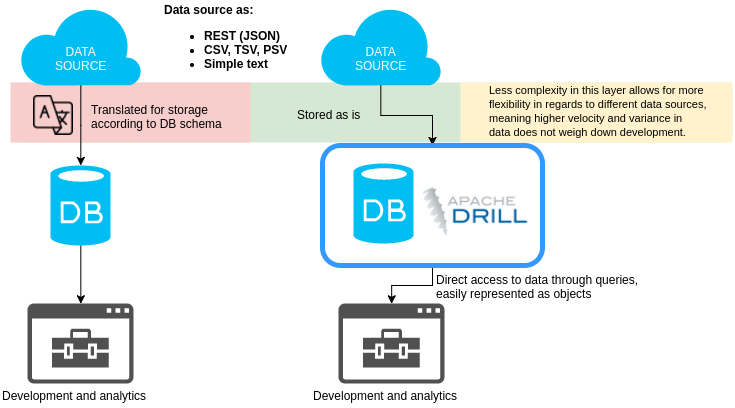
\includegraphics[width=\textwidth]{drill_advantages}
					\caption{Advantages of schema-free querying}
			\end{figure}
			\textit{"Object and relational technologies are grounded in
			different paradigms. Each technology mandates that
			those who use it take a particular view of a universe
			of discourse. Incompatibilities between these views
			manifest as problems of an object-relational
			impedance mismatch"}\cite{impedance}.
			\\
			Traditional databases contain tables (entities) with relations between them. Sometimes these systems consist of thousands of tables, even going as far as tens of thousand (like this database of the human genome with 20000 tables\cite{humangenome}). Object-oriented programming classes is difficult and oftentimes inefficient to map directly to the raw data. Especially when there are large amounts of data, it can take a while just initializing the objects, and then again when serializing them to store them. Adopting complex storage file types like JSON for raw data would overcome this mismatch, and allow for more agile, and reactive development of enterprise applications utilizing huge data sources. The global IT industry is increasingly transitioning to deliver RESTful APIs to their customers. With Apache Drill, it is extremely easy to perform queries on the results, even joining them against several other data sources or combining results from several APIs at the same time, in real time. For application developers this will eliminate the middleware of a relational database, having to translate the data for different purposes. Instead of having one format for storing, one for interfacing and one for application logic, Apache Drill and the schema-free paradigm will provide one single interface for all dimensions of data.
		
		\section{How far will this advance the field?}
			\subsubsection{Advances in research}
			The ambition for this project is to provide a fully functional, open source light weight framework allowing companies to easily deploy Hadoop Clusters with Apache Drill without worrying about tailoring the solution or suboptimal performance. In terms of research, this is the first thesis written about performance tuning of Apache Drill, and as such will lay a foundation for the future of this field.
			\subsubsection{Advances in industry}
			As the previous section highlighted (\hyperref[big_data]{Increasing relevance of Big Data infrastructures}), we predict an increase in future global data collection, going as far as doubling the amount of data per person, per year. This data is only collected to add value to a business, and the revenue increase for businesses that embrace big data analytics will not go unnoticed by the industry, leading to wider adoption. Some businesses already make huge profits simply by gathering and selling information, like Google and Facebook, increasing their yearly revenue since 2011 by 289\% and 1095\% respectively\cite{statista}. Data is becoming the world’s new natural resource\cite{future_data}. To be able to more fluidly handle this data in applications, we believe agile teams will want flexible frameworks that empower more cost effective development and big data utilization. When the industry realizes Apache Drill can deliver that, this will lead to a paradigm shift to schema-free querying of data, and on-the-fly data reads without tailoring.
		
		\section{Structure of the report}
		Add comments about every chapter here.

		
	\chapter{Background}
	\emph{"Apache Drill is one of the fastest growing open source projects, with the community making rapid progress with monthly releases. The key difference is Drill’s agility and flexibility. Along with meeting the table stakes for SQL-on-Hadoop, which is to achieve low latency performance at scale, Drill allows users to analyze the data without any ETL or up-front schema definitions. The data can be in any file format such as text, JSON, or Parquet. Data can have simple types such as strings, integers, dates, or more complex multi-structured data, such as nested maps and arrays. Data can exist in any file system, local or distributed, such as HDFS or S3. Drill, has a “no schema” approach, which enables you to get value from your data in just a few minutes"}\cite{drill}.
	
	\section{History}
		\subsection{Creation and adoption of Hadoop}
		Google created the Google File System in 2003\cite{gfs}, predicting the paradigm of distributed storage. Then, the MapReduce concept for sorting / counting data was added in 2004\cite{mapredoriginal}. Hadoop was introduced as a platform in 2006\cite{hadoopguide}, and together with MapReduce, it made an impact in the industry, attracting talent and big companies eager to contribute and deploy. Yahoo was a big early adopter, being one of the first companies deploying big clusters as early as 2006\cite{hadoopguide}. Then in 2008, Hadoop got the world record for fastest system to sort a terabyte of data\cite{hadoopguide}. After this, development accelerated with more contributers and interest was at an all time high. Since that point in time Apache Hadoop has become the most widely used platform for Big Data handling, empowering advanced analytics and business intelligence across several industries. The Hadoop stack is now highly scalable, ensures high availability of data, and utilizes parallel processing to deliver high performance data readings.
		
		\subsection{Google branching out with Dremel}
		In 2010 Google did further research on distributed data processing and published their paper on Dremel\cite{dremel}. Dremel is the framework that empowers Google's current platform Google BigQuery, delivered as Infrastructure as a Service (IaaS). Among customers of BigQuery is well recognized brands like Spotiy, Coca Cola, Philips, HTC and Niantic\cite{dremelcustomers}. The success of Google BigQuery (by extension of Dremel), inspired Apache to create Drill, the framework being examined in this thesis.
	
	\section{Technology}
	\label{technology}
		
		\subsection{Hadoop stack}
		
		\subsubsection{Hadoop common}
		Hadoop common consists of a few select core libraries, that drives the services and basic processes of Hadoop, such as abstraction of the underlying operating system and file system. It also contains documentation and Java implementation specifications. 
		
		\subsubsection{HDFS}
		HDFS (Hadoop Distributed File System) is a highly fault tolerant, distributed file system designed to run efficiently, even on low-cost hardware. HDFS is tailor made to express large files and huge amounts of data, with high throughput access to application data and high scalability across an arbitrary amount of nodes.
		
		\subsubsection{YARN}
		YARN (Yet Another Resource Negotiator) is actually a set of daemons that run in the cluster to handle how the jobs get distributed. 
		\begin{itemize}
			\item There is a NM (NodeManager) that represents each node in the cluster, monitoring and reporting to the RM whether or not they are idle, and resource usage (CPU, memory, disk, network). A node in a Hadoop cluster divides its resources into abstract Containers, and reports on how many containers there are available for the RM to assign jobs to.
			\item There is an AM (ApplicationMaster) per job, or per chain of jobs, representing the task at hand. This AM gets inserted into containers on nodes, when a job is running.
			\item Finally there is a global RM (ResourceManager), which is the ultimate authority on how to distribute loads and arbitrate resources. The RM consists of two entities, the Scheduler and the ApplicationsManager.
			\begin{itemize}	
				\item The ApplicationsManager is responsible for accepting job submissions (at this point represented as an ApplicationMaster), i.e by doing code verification on submitted jobs, changing their status from "submitted" to "accepted". Once a job is accepted, the ApplicationsManager sends the ApplicationMaster to the scheduler to negotiate and supply containers for the job on the nodes in the cluster. The ApplicationsManager also has services to restart failed ApplicationMasters in containers, and retry entire jobs.
				\item The Scheduler is a pure scheduler in the sense that it only cares about delivering tasks to idle slots, based on free resources on the node. It calculates distributions across multiple nodes / containers, and can prioritize - i.e compute smaller jobs in front of large ones to more effectively complete job queue, even though the large job was submitted first. The Scheduler does not care for monitoring task completions or failures, simply distributing loads on the cluster.
			\end{itemize}
		\end{itemize}
		\textit{The ResourceManager and the NodeManager form the data-computation framework. The per-application ApplicationMaster is, in effect, a framework specific library and is tasked with negotiating resources from the ResourceManager and working with the NodeManager(s) to execute and monitor the tasks}\cite{yarn}.
		
		\subsubsection{MapReduce}
		MapReduce is the heart of a traditional Hadoop cluster, for which every other component is built around, to maximize its efficiency. It is a model for distributed processing of big data, to process and consolidate. It is defined by two stages - the mapping phase, and the reduce phase. Both of these phases require resources from the node it is run on, defined by a set amount of map slots and reduce slots. The amount of slots on a node for each task is parameterized and can be set by an administrator / or typically algorithmically. The map phase consists of parallel map tasks, that map a key to a value. All of these map tasks then consolidate into the reduce phase, where they are combined so that one key exists for all accumulated values. So for instance if we're counting cards in several decks across several nodes, they would each map something like "(Queen of Hearts, 1)". In the end the reduce task consolidates all these single queens, so it ends up looking like "(Queen of Hearts", 27)". This is a far more effective approach than for instance looping through all the decks and incrementing a key by one for each matching key we find. Especially when the data that typically gets handled by a Hadoop cluster is diverse and hard to predict.
		
		\subsection{Zookeeper}
		Zookeeper is not a part of the Hadoop core utilities, but is is often to be found in Hadoop clusters. It is used as a distributed storage platform for configuration information, synchronization and naming. While YARN handles the distribution of tasks between the nodes in the cluster, Zookeper takes care of failover, race conditions and sequential consistency. This tool looks more like orchestration frameworks such as Puppet or Chef, in that it organizes the amount of YARN nodes and distributes configurations, availability and atomicity.
		
		\subsubsection{Zookeeper Quorum}
		Even though Zookeeper is made as a distributed configuration management and failover safeguard, it can be installed on a single node. Running Zookeeper in this way is called a Standalone Operation, and give a user a interface to remotely connect to, to get some data on running services etc. However, we need Zookeper distributed across all our nodes. This is called a Quorum. In a Quorum, every node will check the health of the others. If there is a consensus among nodes that one is down, Zookeeper is able to communicate this to YARN, letting it distribute loads across the remaining healthy nodes. 
		
		\subsection{Apache Drill}
		In this thesis there won't be any in-depth explanations of the inner workings or architecture of Drill, but we'll gloss over the broader picture in this section.
		\subsubsection{What is it}
		Apache drill is the newest technology to be introduced in this chapter. All the previously mentioned frameworks are tried and tested - proven over time. Apache drill rests on top of all these technologies, and provides a way to query almost any non-relational database. This means that we can set up a cluster on a data lake with a very diverse data type, and still perform standard ANSI SQL queries on it. Even in formats like JSON, a simple SQL query can provide all the insights one might need. Apache Drill is inspired by Google Dremel, which as mentioned is the driving force behind their advanced Big Data Analytics tool - Google BigQuery. Apache Drill is a SQL EE for MPP, that works in almost any environment and on almost any file type. Whether querying complex data, text files or entire directories of log files, Apache Drill allows for standard SQL interfaces for reading the data.
		\subsubsection{How does it do it}
		\paragraph{The drillbit}
		In its core Apache Drill simply consists of a Daemon service called a Drillbit. The drillbit can be installed on any server or client device that has data, or on any number of nodes within a Hadoop cluster, to perform SQL queries. This means that Drill is an entirely independent piece of software, able to perform its intended task without any environment specific needs. Thus Drill does not use YARN, and simply uses hadoop for the distributed storage. To run MPP in a cluster however, Drill is dependent on Zookeeper.
		\paragraph{Querying drill} In addition to its flexible installation needs, the query inputs to Drill can come from a wide variety of sources - JDBC, ODBC, a REST interface, and from a C++ or Java API.
		\paragraph{Key components}
		\begin{itemize}
			\item An RPC end point to receive queries and communicate with clients
			\item An SQL parser that interprets the SQL input and outputs a logical plan
			\item An optimizer that takes the logical plan and translates it to a physical plan based on data locality and node resources
			\item A storage engine interface that has the ability to mount any type of storage, from a local hard drive to a distributed storage like HDFS
		\end{itemize}
		\begin{figure}[h]
			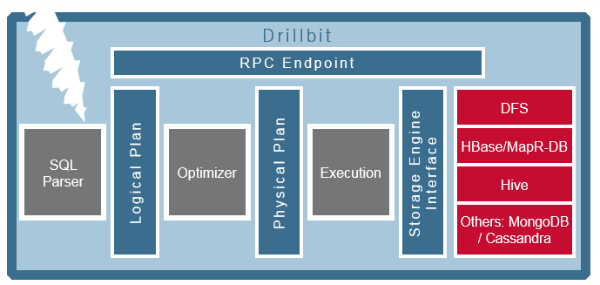
\includegraphics[width=\textwidth]{mapr_drill1}
			\caption{Drill components\cite{mapr_drill}}
		\end{figure}
	
		\paragraph{Drill in a cluster}
		When using Drill as an SQL EE in a distributed storage, it is highly recommended to install a drillbit on all nodes. When set to perform MPP drill is dependent on Zookeeper to keep track of all the drillbits.  When a query is submitted, the first node to respond to the initial request from Zookeeper becomes the \textit{Foreman}. In Drill there is no master or slave hierarchy, and for every query submitted a new foreman is selected. Every drillbit contains all services and capabilities of Drill, which makes it highly scalable - just add another node and install Drill and you're done (after adding it to the Zookeeper Quorum). The foreman gets a list of available Drillbit nodes in the cluster from ZooKeeper, and determines the appropriate nodes to execute various query plan fragments to maximize data locality. This means that Apache Drill both performs the planning, distribution and execution of queries, only depending on Zookeeper to keep track of available nodes. Once a foreman has decided on the distribution of the query, the workload gets split downwards into fragments to the nodes, and the results get consolidated upwards until reaching the foreman, which then returns the results to the client.
		
		\begin{figure}[h]
			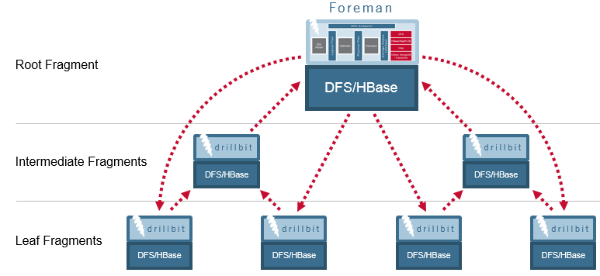
\includegraphics[width=\textwidth]{mapr_drill2}
			\caption{Drill parallel processing\cite{mapr_drill}}
		\end{figure}
		
		\subsection{Drill ODBC Driver, and unixODBC}
		To be able to programatically perform queries to the Drill cluster we need an interface to connect to. This is done via a Open DataBase Connectivity (ODBC), that is installed on the NameNode of the Hadoop cluster. unixODBC is the self-proclaimed definitive standard for ODBC on non MS Windows	platforms\cite{unixodbc}. Once unixODBC was set up, the Drill ODBC Driver was installed on a arbitrary drillbit, although we chose the Hadoop NameNode for this as well. This then allows for setting up a Datasource referencing the Zookeeper Quorum which can then be contacted programmatically, interfacing Drill as if it were a standard SQL server / database.
		
		\subsection{pyodbc}
		There are plenty of ways to interface with an ODBC. We chose python as a preferred language because of familiarity. Therefore we chose to use pyodbc\cite{pyodbc} to communicate with the ODBC, allowing a fully functional interface against our Drill configuration. pyodbc is a well established open source module, implementing the DB API 2.0 specification which is an API defined to encourage similarity between the Python modules that are used to access databases. Defining the Drill ODBC Driver as a datasource, which again points to the Zookeeper Quorum, proved effortless and fast.

		\section{Genetic algorithms}
			\begin{figure}[ht]
				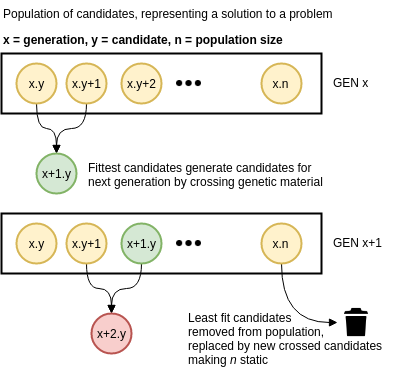
\includegraphics[width=\textwidth]{GA}
				\caption{Basic concepts of GA}
			\end{figure}
			Genetic algorithms are higher level procedures for generating high-quality configurations / solutions to problems with a wide range of parameters, typically where exhaustive searches are infeasible. The procedure starts out with a population of \textit{n} candidates, each representing a set of pseudo-randomly generated values for the respective parameters (properties) that will yield a result for the given problem. Once each candidate has attempted to solve the problem by applying their properties to it, a fitness score is given and compared amongst them. The fitness score represents how good their solution to the problem was, and lets us pick out the best candidates among our population. After the optimal candidates of a generation is chosen, a new generation is generated, inheriting the properties of the previous best candidates. This process repeats until a stop criterion is reached and the properties of the candidate is considered an optimal solution. The number of generations to be generated, and the number of parent candidates from which the next generation is generated from are tweakable parameters.
			
			\subsection{NASA applying genetic algorithms}A very famous application of genetic algorithms is the high-performance antenna NASA made, that actually flew in their Space Technology 5 (ST5) mission\cite{nasa}. In NASAs case, they needed to make a highly receptive antenna with very small physical dimensions. It could have any number of branches, each going in any arbitrary direction. Because of these seemingly infinite possible configurations for the antenna, applying genetic algorithms to gradually evolve a design by testing randomly generated populations and combining the best traits from each candidate, proved to be a great way of solving this. \emph{"(...) the current practice of designing antennas by hand is severely limited because it is both time and labor intensive and requires a significant amount of domain knowledge, evolutionary algorithms can be used to search the design space and automatically find novel antenna designs that are more effective than would otherwise be developed"}\cite{nasa}.
			\subsection{Limitations of genetic algorithms}
			\subsubsection{Fitness function}
			At first glance it sounds like applying genetic algorithm techniques to any problem would yield an optimal solution, with relative ease. The problem though, is the fitness function for determining the candidate solution. As the complexity of the problem scales in size the search space for the fitness function will end up being too big to complete in a reasonable time. For instance if one single candidate evaluation took days, performed for the whole population, across generations, it could end up taking months completing just one single optimization. In those cases machine learning approaches or simply manual labor through technical and domain specific knowledge would prove to be more efficient.
			\subsubsection{Reaching the optimal solution}
			The only way to evaluate a solution is to compare it against other solutions within the population, all of which have are derived from random mutations. Therefore it is impossible to know whether a truly optimal solution is reached, or if one more generation of mutations will prove to give a better result. In practice a stop criterion for the candidate generation is therefore needed, where a solution is considered to be optimal.

	\pagebreak
	\section{Population based incremental learning}
	\begin{figure}[ht]
		\centering
		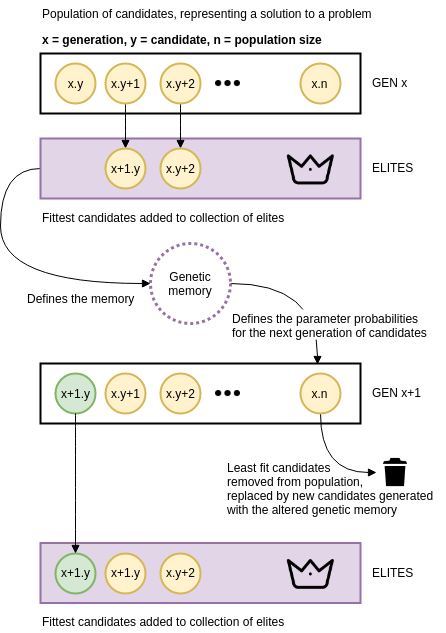
\includegraphics[width=310pt]{PBIL}
		\caption{Basic concepts of PBIL}
	\end{figure}
	The distinction between PBIL and the general GA lies in where the evolution happens. GA generally focus on evolving individual candidates, and crossing fit parents to produce extra fit children, each of them with a chance of mutation. Across several generations convergence is expected. PBIL on the other hand evolves the whole population on a higher level, where the probability vector for parameter generation is shifted towards a considered favorable state. So instead of generating new candidates defined as a crossover function of two parents, the fittest candidates affect a shared genotype that each candidate is generated from. This allows for a much clearer convergence of properties, where you end up in a state where every parameter has a (close to) 100\% chance to be generated. This approach was first proposed back in 1994 by Baluja, where he found that \textit{"The results achieved by PBIL are more accurate and are attained faster than a standard genetic algorithm, both in terms of the number of evaluations performed and the clock speed. The gains in clock speed were achieved because of the simplicity of the algorithm"}\cite{pbil}.
		\subsection{Advantage of PBIL}
		The main advantage PBIL supplies for this problem is the avoidance of unnecessary mutation on key properties, and generally faster convergence. In the case of Apache Drill there are a number of boolean properties that have big impacts on performance, i.e "planner broadcast join" that based on setting can result in a query that is \textit{"(...) substantially cheaper"}\cite{joinplanning}. The impact of flipping this boolean property is based on the type of query being done, the skewness of data locality and cluster size, but for a specific type of query in a set environment the property will always have a strictly optimal value. In PBIL this will become apparent early, and the chance of this value being anything else than the optimal one is likely decreased instantly after first generation run, and in every subsequent run. Typically this will result in a snowballing effect, where crucial parameters quickly get favored, further increasing the chance of them being selected, accelerating the selection process. Further more PBIL allows for complex values as genetic material instead of the usual binary representation, making it easier to implement linear parameters. A shared genetic memory for the population also matches well with the method presented in this thesis - of measuring performance of the candidate parameters on the SQL EE with an authority object. This is further detailed in the \hyperref[sec:judge]{method chapter}.
		\subsection{Limitation of PBIL}
		The main limitation of PBIL is that each candidate property needs a preset of valid values. Thus finding the optimal solution is still based widely on the amount of options, and the effectiveness of them, defined by the developer of the algorithm. Naturally - in terms of boolean properties there lies no challenge. However when linear parameters need to be set, i.e properties with ranges from zero to infinity, the developer must define a set of valid options existing within that range. In the context of Apache Drill there are default rule of thumb values for each property, so the list of valid options for each property is generated around the default.
		Another drawback of PBIL lies in the risk of premature convergence. This can however be mitigated by effective mutation functions that ensure diversity.
	\pagebreak
	\section{Related literature and theoretical focus}
		\subsection{Performance tuning MapReduce as a Research Field}
		There is a ton of research to be read about MapReduce optimization, trying to tune map- and reduce-slots, and improve the inherent job tracker. Looking at a few essential papers within this field shows a general consensus that tuning default performance parameters in a variety of environments will lead to 10-30\% performance increase, which naturally results in considerable cost savings. For instance Min Li et. al. could report that "\textit{Our results using a real implementation on a representative 19-node cluster show that dynamic performance tuning can effectively improve MapReduce application performance by up to 30\% compared to the default configuration used in YARN}"\cite{mronline}. Furthermore, manually tuning these clusters are too demanding for most businesses to even consider, requiring both deep technical and domain-specific insight. These findings further maintain our vision of bringing auto-tuning to the Apache Drill framework, which we believe to be the next natural step forwards, even paradigm-defining, for big data handling.
	
		\subsection{Mapreduce optimization}
			\subsubsection{Gunther}
			Gunther evaluated methods for optimizing Hadoop configurations using machine learning and cost-based models, but found them inadequate for automatic tuning. Thus they introduced a search-based approach with genetic algorithms, designed to identify crucial parameters to reach near-optimal perfomance of the cluster\cite{gunther}. This paper tells us that genetic algorithms as an approach to performance tune big data clusters already is a proven method. However, the scope is set to Hadoop as an out-of-the-box enterprise solution, whereas we take the next step within the schema-on-the-fly paradigm of Apache Drill.
			
			\subsubsection{mrOnline}
			"MapReduce job parameter configuration significantly impacts
			application performance, yet extant implementations place the bur-
			den of tuning the parameters on application programmers. This is
			not ideal, especially because the application developers may not
			have the system-level expertise and information needed to select
			the best configuration. Consequently, the system is utilized inefficiently which leads to degraded application performance"\cite{mronline}.
			
		\subsection{Other Hadoop SQL engines}
		There are plenty of SQL-on-hadoop engines available right now, like CitusDB, Impala, Concurrent Lingual, Hadapt, InfiniDB, JethroData, MammothDB, Apache Drill, MemSQL or Pivotal HawQ, and the amount of independently developed engines speaks volumes of the interest in this field. Why Apache Drill was chosen in this thesis is detailed in the \hyperref[sec:why_drill]{Why Drill section}, but the fact that Drill is (at the time of this writing) the only schema-free engine is a major selling point. However Impala and Spark are often considered as alternatives in similar environments.
			\subsection{Impala}
			Impala, developed by Apache is an opensource SQL engine that was designed to bring parallel DBMS technology to the Hadoop environment\cite{impala}. The main idea is shared between Drill and Impala where they both set up daemons on each node of a distributed cluster, to perform MPP (Massively Parallel Processing) for data reads, circumventing MapReduce. Impala is made for Big Data Analyics, priding itself in having \textit{"order-of-magnitude faster performance than Hive"}\cite{impalasite}.
			\subsection{Spark}
			Apache also developed Spark, a popular open-source platform for large-scale data processing that is	well-suited for iterative machine learning tasks\cite{spark_ml}. Spark is built with Hive, and runs very similarly to MapReduce but also has extended functionality. The key difference is that Spark keeps things in memory, while MapReduce keeps shuffling data in and out of disk. This allows Spark to facilitate machine learning algorithms on top of big data clusters, reading and processing data in the same workflow.
			
	\section{Presentation of domain where technology is used}
		The field of big data analytics is now becoming nigh impossible to ignore for enterprises dealing with customer information. Within this field Hadoop is currently the biggest platform. SiliconANGLE wrote a 5 year future broadcast in 2012, stating that \textit{"Hadoop-MapReduce solution [will] be the de-facto industry standard for business intelligence and projects a 58\% compound annual growth rate"}\cite{siliconA}.
		Global Knowledge Training highlights some of the reasons why Hadoop is seeing such success and adoption rate
		\textit{"It's becoming clear that the open-source Apache Hadoop platform changes the economics and dynamics of large-scale data analytics due to its scalability, cost effectiveness, flexibility, and built-in fault tolerance. It makes possible the massive parallel computing that today's data analysis requires"}\cite{globalknowledge}.
		Further more BMC Software lists industries and sectors where Hadoop is currently being utilized to gain a competitive advantage, increase customer satisfaction or even improve citizen health:
		\begin{itemize}
			\item Financial services companies use analytics to assess risk, build investment models, and create trading algorithms; Hadoop has been used to help build and run those applications\cite{bmc}.
			\item Retailers use it to help analyze structured and unstructured data to better understand and serve their customers\cite{bmc}.
			\item In the asset-intensive energy industry Hadoop-powered analytics are used for predictive maintenance, with input from Internet of Things (IoT) devices feeding data into big data programs\cite{bmc}.
			\item Telecommunications companies can adapt all the aforementioned use cases. For example, they can use Hadoop-powered analytics to execute predictive maintenance on their infrastructure. Big data analytics can also plan efficient network paths and recommend optimal locations for new cell towers or other network expansion. To support customer-facing operations telcos can analyze customer behavior and billing statements to inform new service offerings\cite{bmc}.
			\item There are numerous public sector programs, ranging from anticipating and preventing disease outbreaks to crunching numbers to catch tax cheats\cite{bmc}.
			Hadoop is used in these and other big data programs because it is effective, scalable, and is well supported by large vendor and user communities\cite{bmc}.
			\item Hadoop is a de facto standard in big data\cite{bmc}.
		\end{itemize}
	
		Now it may seem like the Hadoop platform is an all-encompassing 
		technology when businesses wants to deal with big data. There are however some bleaker recent reports stating that Hadoop adoption is going slower than previously predicted. A 2015 Gartner press release stated that \textit{"[the] future demand for Hadoop looks fairly anemic"}\cite{Gartner}. The reasons businesses aren't adopting Hadoop as a big data framework however was fairly coherent, and is also highlighted in this thesis. It is too technically demanding to set up effectively. Companies that were reluctant or hesitant with Hadoop adoption cited skills shortage and user-unfriendliness as reasons for not thinking about Hadoop\cite{Gartner}. This is the exact reason why self optimizing frameworks like the one introduced in this thesis are needed. Making the Hadoop platform more approachable through a "out-of-the-box" mindset could potentially severely lower the threshold for taking a leap into big data. Through the methods presented in this thesis, we try to directly tackle this problem.
	
	\chapter{Method}
		
		\section{Infrastructure}
			To simulate a enterprise environment we set up a cluster consisting of four nodes, each with the same spec - 4 VCPUs and 8GB RAM. These were all VMs in OpenStack, each running Ubuntu 17.10. The cluster is also listed in the appendix, called the \hyperref[table:cluster_shared]{shared cluster} The gateway has a outward-facing network interface for SSH access, and from there each of the other nodes can be managed. They all had Apache Drill installed, and were set up as a Hadoop cluster running HDFS between them. All data that Drill uses to read for tests are replicated three times in the cluster, ensuring parallel processing.
			\begin{figure}[h]
				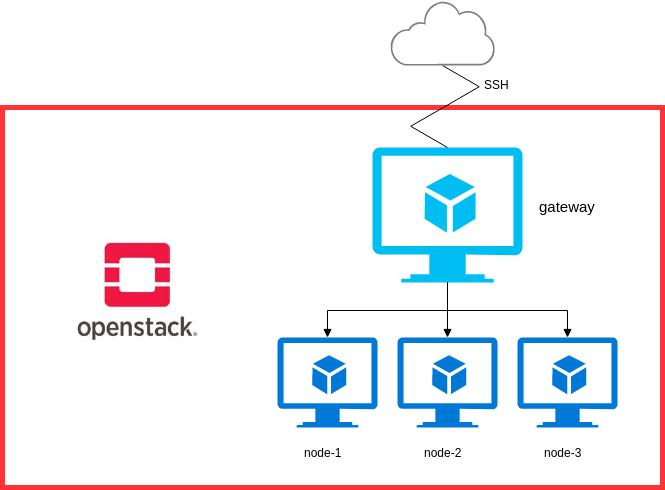
\includegraphics[width=\textwidth]{cluster}
				\caption{Cluster architecture}
			\end{figure}
			The infrastructure stack consists of the technologies listed in the \hyperref[technology]{technology section}. All technologies are installed on all machines, except for the ODBC drivers, that are exclusively on the gateway. During a drill exection, any node can act as the orchestrator, named the \textit{foreman}.
			\begin{figure}[h]
				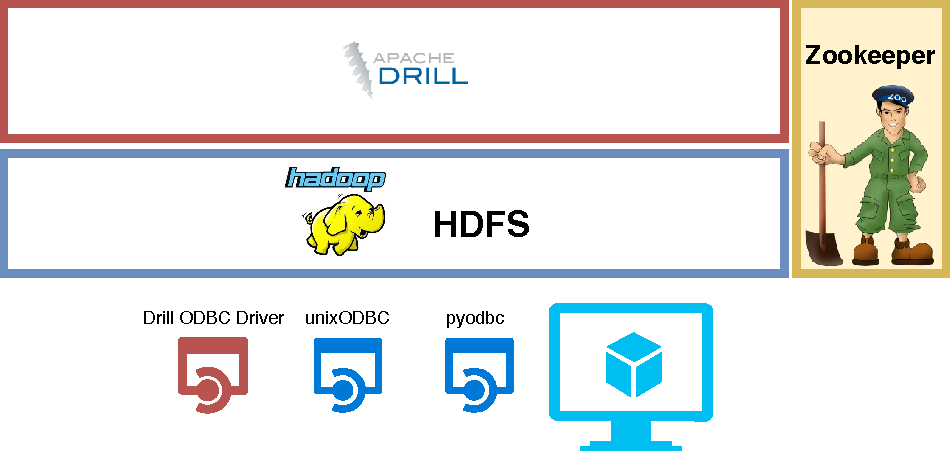
\includegraphics[width=\textwidth]{tech_stack}
				\caption{Technology stack}
			\end{figure}
		\clearpage
		\section{Optimization system overview}
		The overall design of the self optimizer is object oriented, where the judge is the overarching authority in a tree structure. The judge holds the memory and all candidates, and the candidates hold the settings. This makes data easy to keep track of in the optimization process, as everything can be read from the judge.
		\begin{figure}[h]
			\centering
			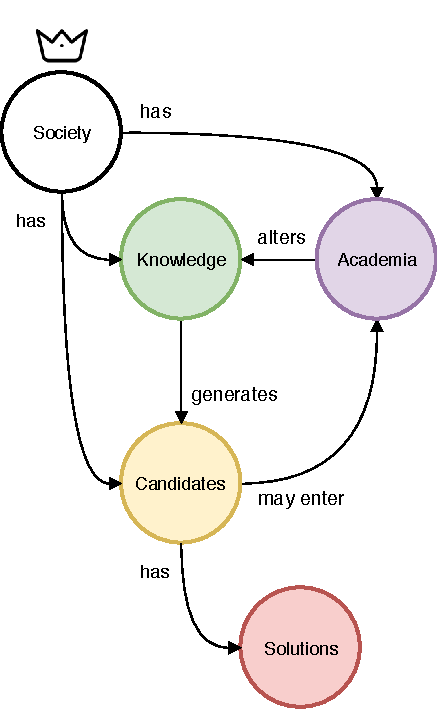
\includegraphics[width=150pt]{OOP}
			\caption{Hierarchy of objects}
		\end{figure}
		\subsection{Judge}
		When initializing a optimization process the first crucial thing to get created is the judge. The judge extracts all of the information contained within the configuration file, to construct itself, the memory object, a default candidate and an initial population.
		\subsubsection{Judge operations}
		\paragraph{Memory}
		The first thing the Judge needs to do, apart from declaring various variables to the itself, is generating a memory object. Without the memory the judge can't initialize any candidates, as they are dependent on the memory to define probability vectors for parameter creations. The global genetic material that defines PBIL is stored in the memory, or rather \textbf{is the memory}. The memory is further explained in the \hyperref[memory]{next subsection.} 
		\paragraph{Default candidate}
		To define goals for the fitness function a candidate is created, with all default values. This candidate also comes into play at the end of a optimization process, to verify solution. In the beginning, the default candidate is simply run the same way as all future solution candidates will, and metrics for mean, maximum and minimum TTE is stored within. The goal is then set at 50\% reduction from the default candidates mean time, giving a somewhat unrealistic goal to ensure that we strive towards the most cost effective solution. In the end we run a gauntlet between the default candidate and the winner (optimal solution), where we measure the averages of all metrics - to ensure that there's no uncontrolled variance that led to the result.
		\paragraph{Population}
		Based on a parameter from the configuration file, the judge generates an entire generation of \textit{n} candidates representing a soluion to the problem. For each generation the judge measures the fitness of all candidates and executes the weakest ones. Then the strongest ones get added to the elite club, which is a set of candidates we call the elites. The elites are the ones that refine the memory, incrementally adapting it and reinforcing good solutions. After the memory has been altered by the newly added elites (and potentially elites that were added earlier), new candidates get added to the population to replace the ones that got executed. The configuration file can drastically alter the way the population behaves, by changing values for operations that are done on each generation:
		\begin{itemize}
			\item The size of the population
			\item The number of elites to add to the club each generation
			\item The number of executions / replacements each generation
			\item The size of the elite club
			   \begin{itemize}
				\item To keep the memory alterations based on fresh new solutions, we want to evict older members. Some versions of PBIL does not include evictions - but for achieving convergence, evictions are crucial.
				\end{itemize}
		\end{itemize}
		\subsection{Memory}
		\label{memory}
		\begin{figure}[h]
			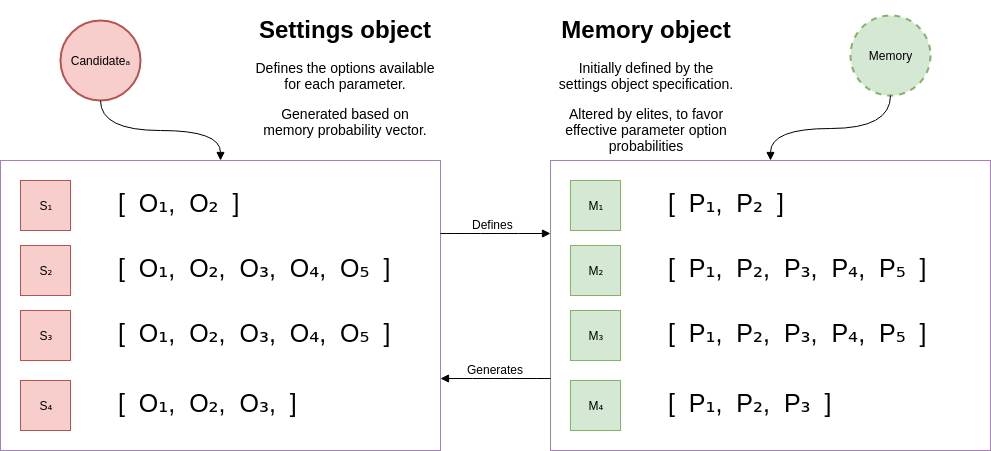
\includegraphics[width=\textwidth]{memory_candidate}
			\caption{The reliance between a candidates' setting object, and the judges' centralized memory.}
		\end{figure}
		The memory is the heart of this entire system. It provides a centralized brain that makes decisions based on historic data, and incrementally adapts it's knowledge as new data is being generated. While it can be considered a machine learning technique, the memory has a truly finite usage within each run, as it is meant to reach a state of convergence. More classic incremental learning schemes are continuously adapting, attempting to for instance predict the stock market. In our case however we simply want to reach one final solution and then end the run. For each run the memory starts out fresh, with a uniformly distributed probability vector, ensuring that changes in i.e cluster topology or data skewness will be taken into consideration when optimizing. Thus it can be valuable to execute one full optimization run each time a big data environment changes, or new data sources get added. If the memory were to store historic genetic material, then certain probability vectors would be skewed in favor of previously strong parameters, that may not be beneficial for current or future runs.
		\clearpage
		\paragraph{Probability vector algorithm}
		\begin{wrapfigure}{r}{5.5cm}
			\caption{How the memory gets altered by the elites}
			\label{fig:memory_insight}
			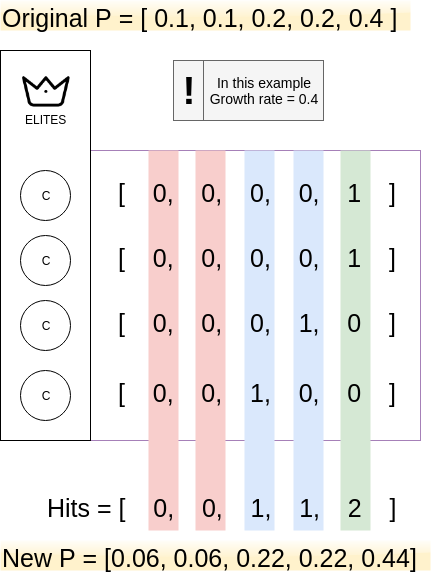
\includegraphics[width=5.5cm]{memory_insight}
		\end{wrapfigure} 
		When altering the memory, we iterate over each elite in the elite club, and view their setting parameters. Each option for a given parameter in the candidate is represented as a list, containing any type of data. The list can be as short or as long as the user likes - it will automatically get a uniform probability distribution in the memory and be eligible for optimization. For each parameter the candidates' setting object contains, there is a mirrored probability vector in memory. When the alterations take place, we check the candidate parameter value and locate it in the list of options, and then return a binary list of hits. For instance if the parameter is boolean the logic would look like this:
		\begin{enumerate}
			\item Parameter value is \textbf{True}
			\item Parameter options are \textbf{[True,False]}
			\item Binary representation will be \textbf{[1,0]}
		\end{enumerate}
		Once this binary option conversion is done for all candidates, we sum up the hits of each option and get a single list for all accumulated hits, as seen in figure \ref{fig:memory_insight}. Finally we can apply the mathematical formula to alter the probability vector, using the accumulated hits list, denoted as:\\
		\begin{math}
			\mathbf{p[i] = p[i] + gr * ( h[i] / e - p[i] )}
		\end{math}\\
		\textit{p = probability, i = index, gr = growth rate, h = hits, e = amount of elites} \\
		
		\paragraph{Accelerated convergence}
		Once the memory convergence value passes 0.8, the memory enters a state of accelerated convergence. In this state the growth factor of the genetic algorithm increases by 0.2. This is due to parameter agnosticism in many queries, and especially in less complex queries or environments. This is further detailed in the discussion section, \hyperref[sec:param_agno]{parameter agnostic queries}.
		
		\paragraph{Extended function - progress}
		The memory object is also responsible for a novel approach to timing genetic algorithm process times. The single biggest drawback of using genetic algorithm techniques for complex problems is execution time, and especially as it's commonly impossible to predict. By tracking convergence values over time, and using a linear regression model to predict when the convergence threshold hits, a suggested progress bar is generated.
		
		\clearpage
		\subsection{Candidate}
		Candidates don't hold much information on their own, as most of it is stored in a setting object, which the candidate holds on to. However the candidate has some crucial functions, like how to run queries with their setting object, how to mutate and how to measure self performance.
		\paragraph{Run}
		To get data on whether or not a particular set of settings will be an effective solution in the current environment, we need to run some tests - here simply defined as runs. To complete a run in this system the candidate is dependent on a data source, and information on how many runs to do, in order to measure the TTE. In a cluster where resources are shared among many users, or multiple queries are ran concurrently on the same quorum, the optimal solution need to take this into consideration. Therefore runs are done in to stages, one for concurrency testing, and another for sequential testing. Both the data source and the number of runs to complete are defined by the configuration file. The data source defines here is a ODBC DSN, but for future work this can be easily altered to point to a JDBC DSN or other similar sources. The number of runs defined by the configuration file is actually doubled in runtime, as it defines both the amount of concurrent runs in addition to the amount of sequentual runs. This means that defining this setting to the absolute minimum of one run, results in two runs - one in the concurrent stage and one in the sequential stage. Performing only a single run would leave too much up to circumstance, in regards to the available resources in the cluster and random error, thus a minimum of two runs is needed to measure performance - although any number higher than this is advised. Further technical details on how the runs are performed can be read in the \hyperref[testing]{testing section}
		
		\paragraph{Mutation}
		To mitigate the issue of premature convergence a mutation function is in place, to mutate new candidates at a set probability defined by the configuration file. After a candidate is created, it may be chosen for mutation. The value that defines the probability for a candidate to be chosen also decides the probability for individual parameters to mutate within the candidates setting object. There is also a resistance value in place, to avoid too heavy mutations, potentially resulting in a useless candidate at later stages, which simply increases the time cost of the algorithm. The resistance value starts at 0, and increases via the resistance growth value set in the configuration file. Each time a parameter is mutated, the resistance growth gets added to the resistance value. It works by linearly reducing the mutation chance for individually chosen candidates. By default this reduction is 1\% per mutation. Increasing the resistance growth would result in more stable candidates, more purely defined by memory, but gives less variations - so this needs to be balanced. A problem that arises with resistance is the fact that iterating over all the settings will lead to heavy skewness of mutating the settings in the start of the object. As mutations happen, the chance for future mutations gets reduced, thus mutating the first setting is likely, while mutating the final setting is highly unlikely. This is dealt with by ensuring that the algorithm chooses a random subset of settings every time, making it just as likely to mutate the end as the start of the settings, instead of iterating from start to end. The mutation is entirely isolated from the memory, and thus chooses a new option for the parameter randomly - even 
		\\
		TODO: Input some math here - like average amount of mutations per candidate, chance of mutating everything, chance of mutating nothing etc - with default settings. \\
		1/5 candidates get chosen, there are 5 replacements each generation.
		There are 29 settings. 1/29, 14 chosen as start on average, and 7 chosen as end on average. Mutation chance is 0.2, 7/0,2 = 1,4 settings mutated on average?
		\\
		\subsection{Setting}
		The setting object is simply a collection of session setting for Apache Drill to apply before running queries. One of the strengths of PBIL is the ability to easily implement linear parameters as opposed to the binary representation of genetic material that GA usually has. As such, each setting is gathered from the documentation from the Apache team, and experimented on to see which ones affect TTE. The full list of parameters can be viewed in \hyperref[system_params]{appendix A}. \\ \hyperref[table:added_params]{Table A.1} shows what parameters where used, that where able to be altered in session. \hyperref[table:removed_params]{Table A.2} shows what parameters had to be cut, due to them only being able to be changed out of session, or them causing segmentation faults. 
		\subsection{Configuration file}
		This thesis focuses on removing the barrier for adoption of big data frameworks. As such one might find it ironic that a configuration file is supplied, that severely impact the performance of the optimization algorithm. However it is expected that the supplied default values set for the algorithm is sufficiently effective for any environment where this is run. With the default values there is a fine balance between execution time of the algorithm, and the margin for how fine grained a optimal solution should be. In addition to this there are very simple guide lines provided, regarding how big the cluster is, how many cores each node has, and how much time to be spent for accuracy sake. All the parameters can be found in \hyperref[table:conf_params]{appendix B}.
		\clearpage
		\subsection{How it all comes together}
		Figure \ref{fig:sys_overview} shows a simplistic flow chart for how the entire system runs, from tart to achieved convergence.
		\begin{figure}[ht]
			\centering
			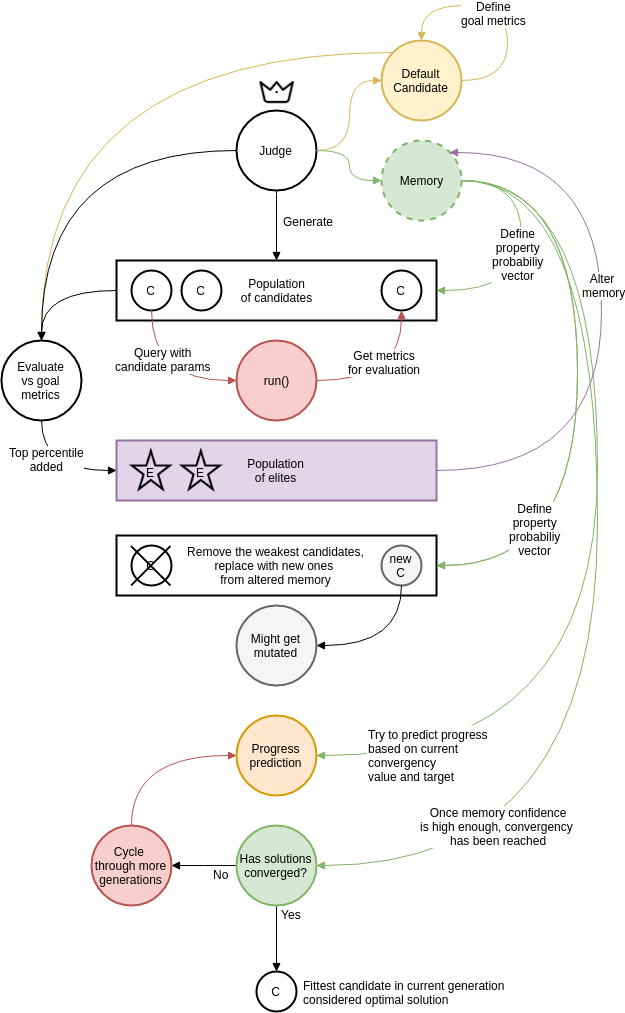
\includegraphics[width=270pt]{overview}
			\caption{System overview}
			\label{fig:sys_overview}
		\end{figure}
		\clearpage
		\section{Testing}
		TODO: This part.
		\label{testing}
			\subsection{Load profiles}
				It should be infeasible for one configuration to solve all problems. After all, the concept of optimization takes great consideration to its specific context. Expecting to solve all aspects of a complex problem with one remedy leads to a candidate being a jack of all trades but master of none. Hence the solution should be tailored to a specific context, by letting the algorithm aggressively tune the system to work in its current state. To make sure this algorithm performs this way, testing was done on different kinds of data sets, with different kinds of queries.
			\subsection{Data collection}
				
	\chapter{Results}
	TODO: this part
	
	\chapter{Discussion}
	\section{The sequential effect}
	As mentioned previously, a candidate run consists of two stages - one concurrent stage and one sequential stage. A single run on a single candidate will always perform at least two sequential queries. All candidates in a population are run in sequence, one after the other whilst measuring their fitness. \textbf{Only elites get counted. always 30\% lower than default, default gets run vs optimal, both perform very bad all of a sudden. What up? Keep this part for now, but do more runs with bigger solution assurance testing pool}
	\section{Parameter agnostic queries}
		\label{sec:param_agno}
		\subsection{Tiny queries}
		Running a very simple query in the cluster environments we set up, on a small json file of a couple thousand lines - took drill around 0.2 seconds. Attempting to optimize for such queries was completely futile, as the only bottleneck for such a simple query is pure hard drive reading speeds. This led to every randomized set of settings to be considered equally good, which again means that the default candidate is equally good. No optimal setting can be discovered, and convergence of the algorithm is simply an act of chance.
		\subsection{Complex queries}
		As queries get more difficult to plan, the data set gets bigger, the cluster gets more heterogeneous and the data source more complex - the impact of performance tuning increases. As discussed previously drill has different phases when executing a query, like the logical and the physical planning phases. The planning phases heavily depend on the configuration settings and performance tuning parameters to calculate how to carry on execution of a query. We discovered early on that in a 4 node cluster with relatively low resources, there were some parameters that heavily impacted the execution time, and some others that were completely arbitrary, or even ignored by drill in runtime. This led to the creation of the accelerated convergence state in the memory object, to increase probability vector growth once the critical parameters have been sorted out. Early proof of concept runs would often see convergence reach around 0.85 - 0.9, before floating back down to around 0.8 and staying there for tens of generations, without ever increasing the fitness value. After introducing accelerated convergence, we give the algorithm an extra push in the higher end of convergence, to make sure we don't waste time and resources on a random gamble of irrelevant parameters.
	\section{Error sources}
		\subsection{Drill planner inconsistency}
		First of all, drill is inherently a bit varied in terms of query times. Performing the same query twice in the same session will heavily leverage a shared cache amongst the drillbits, reducing query times by an average of 15\%. Further more the planning phase contains some fuzzy logic and decision making probabilities, so it may not always result in the same execution stage. The cache issue is mitigated by letting every candidate start a new session, and run the same amount of queries in the session. The planning stage inconsistency is mitigated by running several queries in a single run, to make sure to take the average into consideration. The solutions to both these problems are however parameterized, so setting the amount of queries per run to a low number will lead to increasing impact of these factors as error sources.
		\subsection{Cluster instability}
		In the initial testing phase, results from runs varied widely in execution time. The cluster however, was a shared resource where many projects were competing for computing power. Even running only the default candidate for 50 generations, spikes in TTE as high as 30\% were seen, randomly distributed amongst the runs. This led to a migration to a similar sized cluster of 4 nodes, but with a lower spec, where the resources where allocated and could not be competed for, hereby called the \hyperref[table:cluster_stable]{stable cluster}. This proved effective in terms of mitigating the variations, but still a range of random cost-ineffective candidate runs where observed. When cluster instability gets added on top of drill planner inconsistency in a single query / run, it leads to an outlier of extremely high TTE, which we cut from our dataset when analyzing the data in posterity. With such variations it is hard to reach a sensible convergence for truly optimal solutions, considering how fitness scores then are products of both settings and circumstance.
		\subsection{Cluster size}
		Enterprise environments where optimization techniques like this would be most beneficial, are also the hardest ones to simulate. Increasing the amount of nodes and the amount of resources would add to the complexity, mitigating the optimization problem of parameter agnosticism. 
	\section{Proving effect}
	Considering the error sources at hand, and specifically regarding the cluster instability, it can be difficult to prove that a solution will lead to consistently lower TTE over time - thus saving time and money. Over time a simple solution assurance stage got added to the end of the algorithm, running several runs, 10 by default, where the considered optimal candidate competes against the default candidate. After analyzing this data it is clear that the algorithm works as intended - reducing the overall TTE. Although some error sources will put individual runs from the default candidate ahead of the considered optimal solution in terms of TTE, it is proven across several solution assurance runs that the average cost saving of the suggested optimal solution is worthwhile, averaging out at 20\% for the \hyperref[table:cluster_stable]{stable cluster}, and 5\% for the \hyperref[table:cluster_shared]{shared cluster}. \textbf{TODO: get cost savings right.}
	\section{Cut configuration parameters}
	Time constraints and choice of implemented algorithm caused some relevant parameters to be cut from the optimization process, making them default values in all candidates. There were a total of six cut parameters, viewable in the appendix, \hyperref[table:removed_params]{cut parameters}. The two execution queue memory parameters could not be set in-session, as they were exclusively system settings. This meant that we would need to restart apache for each candidate, to apply their system settings, causing massive overhead and added complexity. The four remaining ones all define what type of aggregation and join functions should be available. Changing these parameters led to segmentation faults while running candidates, and they then had to be cut from the settings list. Given more time, some deeper study and insight could be gained to understand the segmentation faults, and perhaps build systems to handle them.
	
	\chapter{Further work}
	\section{Homogeneous clusters}
	In this thesis both the clusters set up consisted of a homogeneous set of nodes. It is expected that a heterogeneous cluster will have added complexity to the logical and physical planner on the drillbits, further increasing the value of optimization. This is a high priority effort for future work, as it accurately represents a real world use case.
	\section{Single node setups}
	It would be interesting to gather data from a single node laptop setup for running queries in drill. The way data sources work in this thesis through pyodbc meant that it would add too much development time to adapt for local hard drive runs, either in the way of configuring a hard drive location as an ODBC DSN, or altering the way we programatically run drill queries. 
	\section{Support for the cut parameters}
	As mentioned earlier there are a couple of interesting parameters that was cut from the development process in this thesis, listed in \hyperref[table:removed_params]{the appendix}. To handle the segmentation faults potentially caused by hash- and aggregate join disabling, one could possibly access drill through a different source than pyodbc, to create an appropriate wrapper around the runs and catch the errors. To handle the system settings, a more complex run needs to be set up, to restart the cluster and check for readiness before querying it for each candidate - this may ultimately be infeasible in terms of optimization time.
	
	\chapter{Conclusion}
	TODO: this part
	
	\begin{thebibliography}{1}
		\bibitem{mronline}
		Li, M., Zeng, L., Meng, S., Tan, J., Zhang, L., Butt, A. R., \& Fuller, N. (2014, June). \emph{Mronline: Mapreduce online performance tuning. In Proceedings of the 23rd international symposium on High-performance parallel and distributed computing (pp. 165-176).} ACM.
		\bibitem{gunther}
		Liao, G., Datta, K., \& Willke, T. L. (2013, August). \emph{Gunther: Search-based auto-tuning of mapreduce.} In European Conference on Parallel Processing (pp. 406-419). Springer Berlin Heidelberg.
		\bibitem{bmc}
		BMC Software, Inc (2018, January) \emph{http://www.bmc.com/guides/hadoop-examples.html}
		\bibitem{yarn}
		Apache Software Foundation (January 2018) \emph{https://hadoop.apache.org/docs/stable/hadoop-yarn/hadoop-yarn-site/YARN.html}
		\bibitem{starfish}
		Herodotou, H., Lim, H., Luo, G., Borisov, N., Dong, L., Cetin, F. B., \& Babu, S. (2011, January). \emph{Starfish: A Self-tuning System for Big Data Analytics.} In Cidr (Vol. 11, No. 2011, pp. 261-272).
		\bibitem{unixodbc}
		Nick Gorham (2018, February) \emph{http://www.unixodbc.org/}
		\bibitem{pyodbc}
		Michael Kleehammer (2018, February) \emph{https://github.com/mkleehammer/pyodbc}
		\bibitem{hadoopguide}
		White, T. (2012). \emph{Hadoop: The definitive guide.} " O'Reilly Media, Inc.".
		\bibitem{dremel}
		Melnik, S., Gubarev, A., Long, J. J., Romer, G., Shivakumar, S., Tolton, M., \& Vassilakis, T. (2010). \emph{Dremel: interactive analysis of web-scale datasets.} Proceedings of the VLDB Endowment, 3(1-2), 330-339.
		\bibitem{gfs}
		Ghemawat, S., Gobioff, H., \& Leung, S. T. (2003). \emph{The Google file system} (Vol. 37, No. 5, pp. 29-43). ACM.
		\bibitem{mapredoriginal}
		Dean, J., \& Ghemawat, S. (2008). \emph{MapReduce: simplified data processing on large clusters.} Communications of the ACM, 51(1), 107-113.
		\bibitem{dremelcustomers}
		Google LLC (2018, February) \emph{https://cloud.google.com/customers/}
		\bibitem{modis}
		Modis (2018, February) \emph{http://www.modis.com/it-insights/infographics/top-it-jobs-of-2018/}
		\bibitem{own}
		Johannessen, R., Yazidi, A., \& Feng, B. (2017, April). \emph{Hadoop MapReduce scheduling paradigms. In Cloud Computing and Big Data Analysis} (ICCCBDA), 2017 IEEE 2nd International Conference on (pp. 175-179). IEEE.
		\bibitem{nasa}
		Hornby, G., Globus, A., Linden, D., \& Lohn, J. (2006). \emph{Automated antenna design with evolutionary algorithms.} In Space 2006 (p. 7242).
		\bibitem{drill}
		Apache Software Foundation (2018, January) \emph{https://drill.apache.org/docs/analyzing-the-yelp-academic-dataset/}
		\bibitem{joinplanning}
		Apache Software Foundation (2018, January)
		\emph{https://drill.apache.org/docs/join-planning-guidelines/}
		\bibitem{drill_releases}
		Apache Software Foundation (2018, February) 	\emph{https://drill.apache.org/docs/release-notes/}
		\bibitem{impedance}
		Ireland, C., Bowers, D., Newton, M., \& Waugh, K. (2009, March). \emph{A classification of object-relational impedance mismatch.} In Advances in Databases, Knowledge, and Data Applications, 2009. DBKDA'09. First International Conference on (pp. 36-43). IEEE.
		\bibitem{bettercloud}
		2018 BetterCloud Monitor (2018, February)
		\emph{https://www.bettercloud.com/monitor/real-time-enterprise-messaging-comparison-data/}
		\bibitem{humangenome}
		Stack Exchange Inc, posted by user: Thoth (2018, February) \emph{https://stackoverflow.com/questions/42403229/mysql-database-with-thousands-of-tables}
		\bibitem{bigdata}
		Gantz, J., \& Reinsel, D. (2012). \emph{The digital universe in 2020: Big data, bigger digital shadows, and biggest growth in the far east.} IDC iView: IDC Analyze the future, 2007, 1-16
		\bibitem{servicemax}
		Porter, M. E., \& Heppelmann, J. E. (2015). \emph{How smart, connected products are transforming companies.} Harvard Business Review, 93(10), 96-114.
		\bibitem{management_analytics}
		Bendre, M. R., \& Thool, V. R. (2016). \emph{Analytics, challenges and applications in big data environment: a survey.} Journal of Management Analytics, 3(3), 206-239.
		\bibitem{future_data}
		Huang, G., He, J., Chi, C. H., Zhou, W., \& Zhang, Y. (2015, June). \emph{A Data as a Product Model for Future Consumption of Big Stream Data in	Clouds.} In 2015 IEEE International Conference on Services Computing (SCC), (pp. 256-263). IEEE.
		\bibitem{statista}
		Statista, Inc (2018, February) \emph{https://www.statista.com/statistics/ + [266206/googles-annual-global-revenue/, 277229/facebooks-annual-revenue-and-net-income/]}
		\bibitem{no_sql}
		Github user Edlich, curated list (2018, February) \emph{http://nosql-database.org/}
		\bibitem{pbil}
		Baluja, S. (1994). \emph{Population-based incremental learning. a method for integrating genetic search based function optimization and competitive learning} (No. CMU-CS-94-163). Carnegie-Mellon Univ Pittsburgh Pa Dept Of Computer Science.
		\bibitem{impala}
		Bittorf, M. K. A. B. V., Bobrovytsky, T., Erickson, C. C. A. C. J., Hecht, M. G. D., Kuff, M. J. I. J. L., Leblang, D. K. A., ... \& Yoder, M. M. (2015). \emph{Impala: A modern, open-source SQL engine for Hadoop.} In Proceedings of the 7th Biennial Conference on Innovative Data Systems Research.
		\bibitem{impalasite}
		Apache Software Foundation (2018, March) 
		\emph{https://impala.apache.org/overview.html}
		\bibitem{spark_ml}
		Meng, X., Bradley, J., Yavuz, B., Sparks, E., Venkataraman, S., Liu, D., ... \& Xin, D. (2016). \emph{Mllib: Machine learning in apache spark.} The Journal of Machine Learning Research, 17(1), 1235-1241.
		\bibitem{yelp}
		 Yelp Inc. Yelp (2018, March)
		\emph{https://www.yelp.com/dataset/challenge}
		\bibitem{globalknowledge}
		 Global Knowledge Training LLC. (2018, March)\\
		 Big Data and Apache Hadoop Adoption: Key Challenges and Rewards
		\emph{https://www.globalknowledge.com/us-en/content/articles/big-data-and-apache-hadoop-adoption/}
		\bibitem{siliconA}
		SiliconANGLE Media, Inc. (2018, March)
		\emph{https://siliconangle.com/blog/2012/08/01/hadoop-big-data-reports-future-growth/}
		\bibitem{Gartner}
		Gartner, Inc, Gartner Survey Highlights Challenges to Hadoop Adoption
		\emph{https://www.gartner.com/newsroom/id/3051717} STAMFORD, Conn., May 13, 2015
		\bibitem{mapr_drill}
		MapR Technologies, Inc. (2018, March)
		\emph{https://mapr.com/blog/apache-drill-architecture-ultimate-guide/}
	\end{thebibliography}

\appendix
\chapter{Cluster specs}
\begin{table}[ht]
	\centering
	\caption{Specs for the shared cluster}
	\label{table:cluster_shared}
	\begin{tabular}{ll}
		\\
		\multicolumn{1}{l}{\bfseries Specification} & \multicolumn{1}{l}{\bfseries Value} \\ \hline \\
		Amount of nodes & 4  \\
		Heterogeneous & No  \\
		OS & Ubuntu 17.10  \\
		VCPUs & 4  \\
		RAM & 8GB  \\ 
		HDD & 80GB  \\
	\end{tabular}
\end{table}

\begin{table}[ht]
	\centering
	\caption{Specs for the stable cluster}
	\label{table:cluster_stable}
	\begin{tabular}{ll}
		\\
		\multicolumn{1}{l}{\bfseries Specification} & \multicolumn{1}{l}{\bfseries Value} \\ \hline \\
		Amount of nodes & 4  \\
		Heterogeneous & No  \\
		OS & Ubuntu 16.04  \\
		VCPUs & 2  \\
		RAM & 2GB  \\ 
		HDD & 15GB  \\
	\end{tabular}
\end{table}

\chapter{System parameters}
\label{system_params}
\begin{table}[ht]
	\centering
	\caption{All parameters and options used by PBIL in this thesis}
	\label{table:added_params}
	\begin{tabular}{ll}
		\\
		\multicolumn{1}{l}{\bfseries Name} & \multicolumn{1}{l}{\bfseries Default value} \\ \hline \\
		planner.memory.enable\_memory\_estimation & False  \\
		exec.queue.enable & False  \\
		planner.broadcast\_factor & 1  \\
		planner.broadcast\_threshold & 10000000  \\
		planner.slice\_target & 1000  \\
		planner.width.max\_per\_query & 1000  \\
		exec.min\_hash\_table\_size & 65536  \\
		exec.max\_hash\_table\_size & 1073741824  \\
		exec.queue.large & 10  \\
		exec.queue.small & 100  \\
		exec.queue.threshold & 30000000  \\
		exec.queue.timeout\_millis & 300000  \\
		planner.memory.max\_query\_memory\_per\_node &  max\_query\_memory  \\
		planner.width.max\_per\_node & calculated  \\
		planner.add\_producer\_consumer & False  \\
		planner.enable\_hashjoin\_swap & True  \\
		planner.enable\_mergejoin & True  \\
		planner.filter.max\_selectivity\_estimate\_factor & 1  \\
		planner.filter.min\_selectivity\_estimate\_factor & 0  \\
		planner.join.hash\_join\_swap\_margin\_factor & 10  \\
		planner.join.row\_count\_estimate\_factor & 1  \\
		planner.memory.average\_field\_width & 8  \\
		planner.memory.hash\_agg\_table\_factor & 1.1  \\
		planner.memory.hash\_join\_table\_factor & 1.1  \\
		planner.memory.non\_blocking\_operators\_memory & 64  \\
		planner.partitioner\_sender\_max\_threads & 8  \\
		planner.nestedloopjoin\_factor & 100  \\
		planner.producer\_consumer\_queue\_size & 10  \\
		store.text.estimated\_row\_size\_bytes & 100  \\
	\end{tabular}
\end{table}

\begin{table}[ht]
	\centering
	\caption{Parameters and options that was removed during development, but still is considered to have impact on performance of query execution}
	\label{table:removed_params}
	\begin{tabular}{ll}
		\\
		\multicolumn{1}{l}{\bfseries Name} & \multicolumn{1}{l}{\bfseries Default value} \\ \hline \\
		planner.enable\_multiphase\_agg & True  \\
		planner.enable\_broadcast\_join & True  \\
		planner.enable\_hashagg & True  \\
		planner.enable\_hashjoin & True  \\
		exec.queue.memory\_ratio & 10  \\ 
		exec.queue.memory\_reserve\_ratio & 0.2  \\
	\end{tabular}
\end{table}

\chapter{Configuration parameters}
\begin{table}[ht]
	\centering
	\caption{Configuration parameters that define how the algorithm executes.}
	\label{table:conf_params}
	\begin{tabular}{ll}
		\\
		\multicolumn{1}{l}{\bfseries Name} & \multicolumn{1}{l}{\bfseries Default value} \\ \hline \\
		Parameter & Value  \\
	\end{tabular}
\end{table}

\chapter{Code}
\end{document}